\documentclass[12pt,a4paper]{report}
\usepackage[utf8]{inputenc}
\usepackage[english]{babel}
\usepackage{geometry}
\usepackage{graphicx}
\usepackage{fancyhdr}
\usepackage{titlesec}
\usepackage{xcolor}
\usepackage{hyperref}
\usepackage{listings}
\usepackage{caption}
\usepackage{float}
\usepackage{tcolorbox}
\usepackage{booktabs}
\usepackage{tikz}
\usetikzlibrary{shapes,arrows,positioning,shadows}

\geometry{left=2.5cm, right=2.5cm, top=3cm, bottom=3cm}

\definecolor{primarycolor}{RGB}{26,188,156}
\definecolor{secondarycolor}{RGB}{102,126,234}

\hypersetup{colorlinks=true, linkcolor=primarycolor, urlcolor=blue}

\titleformat{\chapter}[display]{\normalfont\huge\bfseries\color{primarycolor}}{\chaptertitlename\ \thechapter}{20pt}{\Huge}
\titleformat{\section}{\normalfont\Large\bfseries\color{secondarycolor}}{\thesection}{1em}{}

\pagestyle{fancy}
\fancyhf{}
\fancyhead[L]{\leftmark}
\fancyhead[R]{\thepage}

\begin{document}

% TITLE PAGE
\begin{titlepage}
    \centering
    \begin{minipage}[t]{0.3\textwidth}
        \flushleft
        \includegraphics[width=\textwidth]{report_images/image.png}
    \end{minipage}%
    \hfill
    \begin{minipage}[t]{0.3\textwidth}
        \flushright
        \includegraphics[width=\textwidth]{report_images/image.png}
    \end{minipage}
    
    \vspace{3cm}
    {\Huge\bfseries\color{primarycolor} Vehicle Inspection System\par}
    \vspace{0.5cm}
    {\Large\color{secondarycolor} Web-Based Inspection Management Platform\par}
    \vspace{2cm}
    {\Large\textbf{Realized by:}\par}
    \vspace{0.5cm}
    {\large Your Name\par}
    {\large Student ID: XXXXXXXX\par}
    \vspace{2cm}
    {\large Department of Computer Science\par}
    {\large Your University Name\par}
    \vfill
    {\large Academic Year 2024-2025\par}
    {\large \today\par}
\end{titlepage}

\tableofcontents
\newpage

% ABSTRACT
\chapter*{Abstract}
\addcontentsline{toc}{chapter}{Abstract}

This report presents a comprehensive Vehicle Inspection System developed as a modern web-based platform. The system implements a microservices architecture with seven independent services: authentication, appointments, payments, inspections, logging, notifications, and file management. The platform serves customers, technicians, and administrators with features including online booking, secure payments, PDF certificates, photo uploads, and real-time notifications. Built with FastAPI and PostgreSQL, the system demonstrates modern practices in API design, security, and user experience.

\textbf{Keywords:} Vehicle Inspection, Microservices, FastAPI, PostgreSQL, Web Application

\newpage

% CHAPTER 1: INTRODUCTION
\chapter{Introduction}

\section{Context and Motivation}
Vehicle inspection is critical for road safety and environmental compliance. Traditional centers face challenges with manual processes, paper records, and inefficient communication. This project modernizes the inspection process through digital automation and centralized management.

\section{Objectives}
\begin{itemize}
    \item Develop a web-based inspection management platform
    \item Implement microservices architecture for scalability
    \item Provide role-based access (customer, technician, admin)
    \item Enable online booking and payment processing
    \item Generate digital PDF certificates
    \item Implement real-time notifications
    \item Support photo documentation
\end{itemize}

% CHAPTER 2: ARCHITECTURE
\chapter{System Architecture}

\section{High-Level Design}

\begin{figure}[H]
\centering
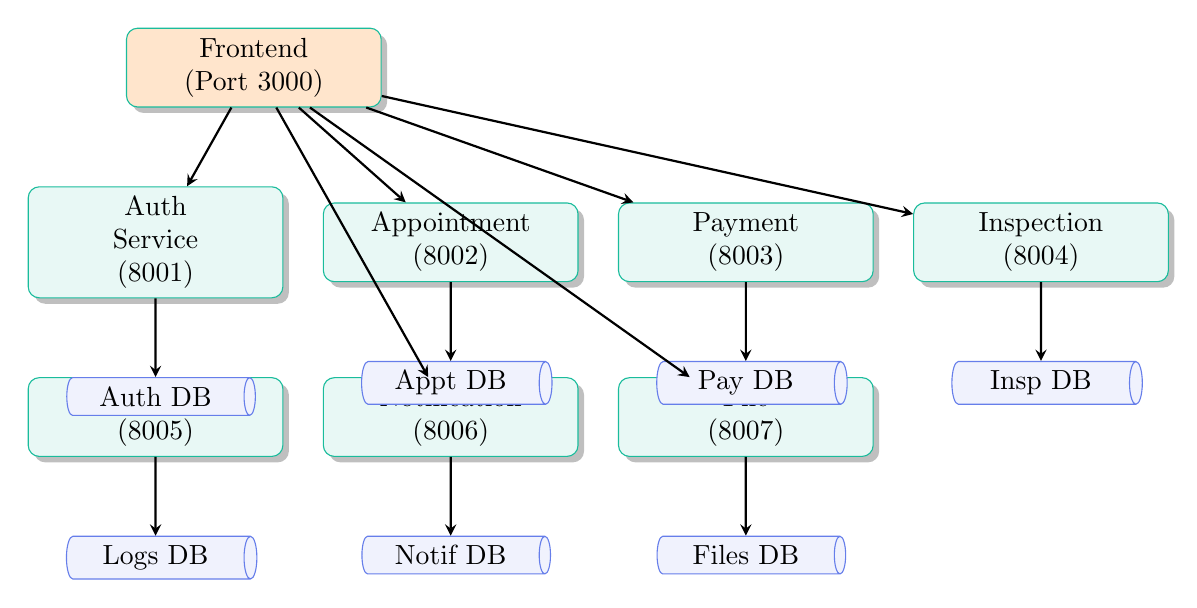
\begin{tikzpicture}[
    node distance=1.5cm,
    service/.style={rectangle, rounded corners, draw=primarycolor, fill=primarycolor!10, text width=3cm, text centered, minimum height=1cm, drop shadow},
    db/.style={cylinder, draw=secondarycolor, fill=secondarycolor!10, text width=2cm, text centered, minimum height=0.8cm, shape aspect=0.3},
    arrow/.style={->, thick, >=stealth}
]

% Frontend
\node[service, fill=orange!20] (frontend) {Frontend\\(Port 3000)};

% Services layer
\node[service, below left=1cm and -2cm of frontend] (auth) {Auth\\Service\\(8001)};
\node[service, right=0.5cm of auth] (appt) {Appointment\\(8002)};
\node[service, right=0.5cm of appt] (pay) {Payment\\(8003)};
\node[service, right=0.5cm of pay] (insp) {Inspection\\(8004)};

% Second row services
\node[service, below=1cm of auth] (log) {Logging\\(8005)};
\node[service, right=0.5cm of log] (notif) {Notification\\(8006)};
\node[service, right=0.5cm of notif] (file) {File\\(8007)};

% Databases
\node[db, below=1cm of log] (db1) {Logs DB};
\node[db, below=1cm of notif] (db2) {Notif DB};
\node[db, below=1cm of file] (db3) {Files DB};
\node[db, below=1cm of auth] (db4) {Auth DB};
\node[db, below=1cm of appt] (db5) {Appt DB};
\node[db, below=1cm of pay] (db6) {Pay DB};
\node[db, below=1cm of insp] (db7) {Insp DB};

% Arrows
\draw[arrow] (frontend) -- (auth);
\draw[arrow] (frontend) -- (appt);
\draw[arrow] (frontend) -- (pay);
\draw[arrow] (frontend) -- (insp);
\draw[arrow] (frontend) -- (notif);
\draw[arrow] (frontend) -- (file);

\draw[arrow] (auth) -- (db4);
\draw[arrow] (appt) -- (db5);
\draw[arrow] (pay) -- (db6);
\draw[arrow] (insp) -- (db7);
\draw[arrow] (log) -- (db1);
\draw[arrow] (notif) -- (db2);
\draw[arrow] (file) -- (db3);

\end{tikzpicture}
\caption{System High-Level Architecture}
\label{fig:architecture}
\end{figure}

\section{Microservices Overview}

\begin{table}[H]
\centering
\caption{Microservices Description}
\begin{tabular}{lcp{7cm}}
\toprule
\textbf{Service} & \textbf{Port} & \textbf{Functionality} \\
\midrule
Auth & 8001 & User registration, login, JWT tokens \\
Appointment & 8002 & Booking, scheduling, availability \\
Payment & 8003 & Payment processing, transactions \\
Inspection & 8004 & Inspection results, PDF generation \\
Logging & 8005 & Centralized event logging \\
Notification & 8006 & Real-time notifications \\
File & 8007 & Photo uploads, file storage \\
Frontend & 3000 & User interface (SPA) \\
\bottomrule
\end{tabular}
\end{table}

% CHAPTER 3: TECHNOLOGIES
\chapter{Technologies}

\section{Backend Stack}
\begin{itemize}
    \item \textbf{FastAPI:} Modern async web framework
    \item \textbf{PostgreSQL:} Relational database (7 databases)
    \item \textbf{SQLAlchemy:} ORM with async support
    \item \textbf{PyJWT:} JWT authentication
    \item \textbf{bcrypt:} Password hashing
    \item \textbf{httpx:} Inter-service HTTP communication
    \item \textbf{reportlab:} PDF generation
\end{itemize}

\section{Frontend Stack}
\begin{itemize}
    \item \textbf{HTML5/CSS3:} Structure and styling
    \item \textbf{JavaScript (ES6+):} Dynamic functionality
    \item \textbf{Fetch API:} HTTP requests
\end{itemize}

% CHAPTER 4: FEATURES
\chapter{Features and Functionality}

\section{Authentication System}

\begin{figure}[H]
\centering
\includegraphics[width=0.8\textwidth]{report_images/login_full.png}
\caption{Login Interface}
\end{figure}

Features:
\begin{itemize}
    \item Secure registration with validation
    \item JWT-based authentication
    \item Role-based access control (Customer, Technician, Admin)
    \item Password encryption with bcrypt
\end{itemize}

\section{Customer Features}

\subsection{Dashboard and Scheduling}
\begin{figure}[H]
\centering
\includegraphics[width=0.9\textwidth]{report_images/customer_dashboard_schedule_appoi.png}
\caption{Customer Dashboard - Weekly Schedule}
\end{figure}

\subsection{Appointment Booking}
\begin{figure}[H]
\centering
\includegraphics[width=0.8\textwidth]{report_images/customer_making_appointment.png}
\caption{Creating New Appointment}
\end{figure}

\subsection{Payment Processing}
\begin{figure}[H]
\centering
\includegraphics[width=0.7\textwidth]{report_images/appointment_to_be_paid.png}
\caption{Appointment Awaiting Payment}
\end{figure}

\begin{figure}[H]
\centering
\includegraphics[width=0.7\textwidth]{report_images/paid.png}
\caption{Payment Confirmation}
\end{figure}

\subsection{Inspection Results}
\begin{figure}[H]
\centering
\includegraphics[width=0.9\textwidth]{report_images/customer_results_inspection.png}
\caption{Customer Inspection Results View}
\end{figure}

\begin{figure}[H]
\centering
\includegraphics[width=0.8\textwidth]{report_images/inspection_details_customer.png}
\caption{Detailed Inspection View with Photos}
\end{figure}

\subsection{Notifications}
\begin{figure}[H]
\centering
\includegraphics[width=0.8\textwidth]{report_images/notifications_for_customer_appointment_payment.png}
\caption{Real-time Notifications System}
\end{figure}

\section{Technician Features}

\subsection{Inspection Dashboard}
\begin{figure}[H]
\centering
\includegraphics[width=0.9\textwidth]{report_images/technician_dashboard_inspection.png}
\caption{Technician Dashboard - Vehicles List}
\end{figure}

\subsection{Inspection Submission}
\begin{figure}[H]
\centering
\includegraphics[width=0.9\textwidth]{report_images/submit_inspection.png}
\caption{Inspection Form with Photo Upload}
\end{figure}

\begin{figure}[H]
\centering
\includegraphics[width=0.7\textwidth]{report_images/inspection_submitted_successful.png}
\caption{Successful Inspection Submission}
\end{figure}

\section{Administrator Features}

\subsection{User Management}
\begin{figure}[H]
\centering
\includegraphics[width=0.9\textwidth]{report_images/admin_dashboard_users_management.png}
\caption{Admin - User Management}
\end{figure}

\subsection{Vehicle Management}
\begin{figure}[H]
\centering
\includegraphics[width=0.9\textwidth]{report_images/vehicules_admin.png}
\caption{Admin - Vehicle Overview}
\end{figure}

\subsection{Appointments Overview}
\begin{figure}[H]
\centering
\includegraphics[width=0.9\textwidth]{report_images/appointments_admin.png}
\caption{Admin - Appointments Management}
\end{figure}

\subsection{Inspections Monitoring}
\begin{figure}[H]
\centering
\includegraphics[width=0.9\textwidth]{report_images/admin_inspections.png}
\caption{Admin - Inspections Overview}
\end{figure}

\subsection{System Logs}
\begin{figure}[H]
\centering
\includegraphics[width=0.9\textwidth]{report_images/admin_logs.png}
\caption{Admin - System Logs}
\end{figure}

\subsection{Schedule Management}
\begin{figure}[H]
\centering
\includegraphics[width=0.9\textwidth]{report_images/admin_schedule.png}
\caption{Admin - Weekly Schedule View}
\end{figure}

% CHAPTER 5: DATABASE
\chapter{Database Design}

\section{Database Schema}
The system uses 7 PostgreSQL databases:

\subsection{Auth Database}
\begin{itemize}
    \item \textbf{users:} id, email, password\_hash, role, first\_name, last\_name, birthdate, country, state, id\_number
\end{itemize}

\subsection{Appointments Database}
\begin{itemize}
    \item \textbf{appointments:} id, user\_id, vehicle\_info (JSON), appointment\_time, status, payment\_status
\end{itemize}

\subsection{Inspections Database}
\begin{itemize}
    \item \textbf{inspections:} id, appointment\_id, technician\_id, results (JSON), final\_status, notes, created\_at
\end{itemize}

\subsection{Payments Database}
\begin{itemize}
    \item \textbf{payments:} id, appointment\_id, amount, status, transaction\_id, created\_at
\end{itemize}

\subsection{Notifications Database}
\begin{itemize}
    \item \textbf{notifications:} id, user\_id, subject, message, is\_read, sent\_at
\end{itemize}

\subsection{Files Database}
\begin{itemize}
    \item \textbf{file\_uploads:} id, appointment\_id, inspection\_id, filename, file\_path, uploaded\_at
\end{itemize}

\subsection{Logs Database}
\begin{itemize}
    \item \textbf{logs:} id, service, event\_type, level, message, timestamp
\end{itemize}

% CHAPTER 6: IMPLEMENTATION
\chapter{Implementation Details}

\section{Security Features}
\begin{itemize}
    \item JWT-based authentication
    \item Password hashing with bcrypt (cost factor 12)
    \item Role-based authorization
    \item CORS protection
    \item Input validation with Pydantic
    \item SQL injection prevention via ORM
\end{itemize}

\section{Key Algorithms}

\subsection{Inspection Status Calculation}
The system determines final inspection status based on individual item results:
\begin{itemize}
    \item All items PASS → Status: \texttt{passed}
    \item Any item FAIL → Status: \texttt{failed}
    \item Mixed results → Status: \texttt{passed\_with\_minor\_issues}
\end{itemize}

\subsection{Notification Targeting}
Notifications are sent to specific users:
\begin{itemize}
    \item Registration → User receives welcome notification
    \item Appointment → Customer receives confirmation
    \item Payment → Customer receives receipt
    \item Inspection complete → Vehicle owner receives results
\end{itemize}

\section{PDF Generation}
Uses reportlab library to generate professional certificates including:
\begin{itemize}
    \item Vehicle information
    \item Inspection results with color coding
    \item Inspector notes
    \item Generated timestamp
    \item Color-coded status banner
\end{itemize}

% CHAPTER 7: TESTING
\chapter{Testing and Validation}

\section{Testing Methodology}
\begin{itemize}
    \item \textbf{Unit Testing:} Individual service endpoints
    \item \textbf{Integration Testing:} Inter-service communication
    \item \textbf{User Acceptance Testing:} End-to-end workflows
    \item \textbf{Security Testing:} Authentication and authorization
\end{itemize}

\section{Test Scenarios}
\begin{enumerate}
    \item Customer registration and login
    \item Appointment booking and payment
    \item Technician inspection submission
    \item Admin monitoring and management
    \item Notification delivery
    \item PDF certificate generation
    \item File upload and retrieval
\end{enumerate}

\section{Performance Metrics}
\begin{itemize}
    \item Average response time: < 200ms
    \item Database query optimization with indexes
    \item Async operations for non-blocking I/O
    \item Connection pooling for database efficiency
\end{itemize}

% CHAPTER 8: CONCLUSION
\chapter{Conclusion and Future Work}

\section{Achievements}
This project successfully delivered a complete vehicle inspection management system with:
\begin{itemize}
    \item 7 independent microservices
    \item 3 user roles with distinct functionalities
    \item Real-time notifications
    \item Secure payment processing
    \item PDF certificate generation
    \item Photo documentation
    \item Comprehensive admin monitoring
\end{itemize}

\section{Challenges Overcome}
\begin{itemize}
    \item Inter-service communication and data consistency
    \item Real-time notification implementation
    \item Role-based access control across services
    \item PDF generation with professional formatting
    \item Error handling and user feedback
\end{itemize}

\section{Future Enhancements}
\begin{itemize}
    \item SMS and email notifications
    \item Online payment integration (Stripe/PayPal)
    \item Mobile application (React Native)
    \item Advanced analytics and reporting
    \item Multi-language support
    \item Appointment reminders
    \item Rating system for technicians
    \item Integration with government databases
\end{itemize}

\section{Lessons Learned}
\begin{itemize}
    \item Microservices provide flexibility but require careful design
    \item Security must be considered from the start
    \item User experience is crucial for adoption
    \item Testing is essential for reliability
    \item Documentation facilitates maintenance
\end{itemize}

% REFERENCES
\begin{thebibliography}{9}

\bibitem{fastapi}
FastAPI Documentation,
\textit{https://fastapi.tiangolo.com/},
Accessed: 2025

\bibitem{sqlalchemy}
SQLAlchemy Documentation,
\textit{https://www.sqlalchemy.org/},
Accessed: 2025

\bibitem{postgresql}
PostgreSQL Documentation,
\textit{https://www.postgresql.org/docs/},
Accessed: 2025

\bibitem{jwt}
JWT.io - JSON Web Tokens,
\textit{https://jwt.io/},
Accessed: 2025

\bibitem{microservices}
Richardson, Chris,
\textit{Microservices Patterns},
Manning Publications, 2018

\end{thebibliography}

\end{document}
